\begin{figure}[H]
\centering
\includegraphics[page=6,width=0.48\textwidth]{\FCNCFigures/tthML/showFake/faketau/postfit/NOMINAL_closureTest/lowBDT_reg1l1tau1b1j_ss_vetobtagwp70_highmet/lep_pt_0.pdf}
\includegraphics[page=6,width=0.48\textwidth]{\FCNCFigures/tthML/showFake/faketau/postfit/NOMINAL_closureTest/lowBDT_reg1l1tau1b2j_ss_vetobtagwp70_highmet/lep_pt_0.pdf}

\includegraphics[page=6,width=0.48\textwidth]{\FCNCFigures/tthML/showFake/faketau/postfit/NOMINAL_closureTest/lowBDT_reg1l1tau1b2j_os_vetobtagwp70_highmet/lep_pt_0.pdf}
\includegraphics[page=6,width=0.48\textwidth]{\FCNCFigures/tthML/showFake/faketau/postfit/NOMINAL_closureTest/lowBDT_reg1l1tau1b3j_os_vetobtagwp70_highmet/lep_pt_0.pdf}

\caption{用于ABCD方法闭合测试的lowBDT控制区的轻子$\pt$谱,图中未考虑任何系统误差(ABCD方法的系统误差也未考虑),数据和本底估计已经符合得较好,因此不需要额外加入系统误差。}
\label{fig:closuretest}
\end{figure}
